\documentclass[border=0pt]{standalone}
\usepackage{tikz}
\usetikzlibrary{decorations.pathreplacing,
  arrows,
  calc,
  decorations.pathmorphing,
  decorations.pathreplacing,
  decorations.markings,
  fadings,
  positioning,
  shapes,
  3d
}
\tikzfading[name=fade img right,left color=transparent!100, right color=transparent!0]
\tikzfading[name=fade img left,right color=transparent!100, left color=transparent!0]
\tikzstyle{snakearrow} = [decorate, decoration={pre length=0.1cm,
  post length=0.1cm, snake, amplitude=.4mm,
  segment length=4mm},thick, ->]
\usepackage{graphicx}
\begin{document}
\newcommand*{\arrowthreeD}[5]{%
  \fill[left color=#1!50!black,right color=#1!50!black,middle color=#1!43,
  shift = {#2},
  opacity=0.9,
  rotate=#3,shading=axis,shading angle=90+#3]
  (0,0) -- (83:#4) arc (83:97:#4) -- cycle;
  \fill[left color=#1!50!black,right color=#1!50!black,middle color=#1!43,
  shift = {#2},
  opacity=0.9,
  rotate=#3,shading=axis,shading angle=90+#3]
  (87:#4) -- ++(0, #5) -- ++(-{2 * #4 * sin(3)}, 0) -- (93:#4) -- cycle;
}
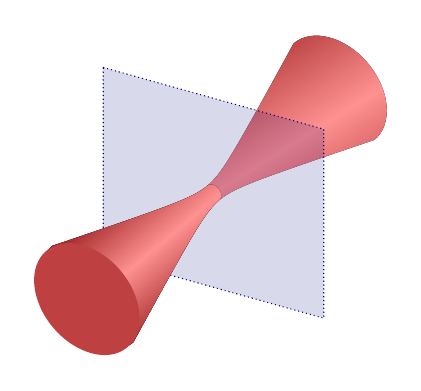
\begin{tikzpicture}
  \pgfmathsetmacro{\radiush}{0.8}
  \pgfmathsetmacro{\theight}{2}
  \pgfmathsetmacro{\radiusv}{.7 * \radiush}
  \pgfmathsetmacro{\waist}{.15}
  \pgfmathsetmacro{\xscale}{\radiush / sqrt(1 + (\waist)^2)}

  \fill[left color=red!50!black,right color=red!50!black,middle color=red!43,
  shading=axis,rotate=-50,shading angle=32]
  plot[domain={-1}:{1}, smooth, variable=\y] ({sqrt((\y)^2 + (\waist)^2) * \xscale}, \y * \theight)
  arc (0:180:\radiush cm and \radiusv cm)
  -- plot[domain={-1}:{1}, smooth, variable=\y] ({-sqrt((\y)^2 + (\waist)^2) * \xscale}, -\y * \theight)
  arc (180:360:\radiush cm and \radiusv cm);

  \arrowthreeD{orange}{(0.3, 0)}{-90}{0.3}{1.2};

  \begin{scope}[transform canvas={cm={1,-0.28,0,1,(0, 0)}}]
    \fill[blue!50!black,opacity=0.15] (-1.4, 1.2) -- (1.4, 1.2)
    -- (1.4, -1.2) -- (-1.4, -1.2) -- cycle;
    \draw[blue!50!black, densely dotted] (-1.4, 1.2) -- (1.4, 1.2)
    -- (1.4, -1.2) -- (-1.4, -1.2) -- cycle;
    \arrowthreeD{red}{(0, -0.2)}{180}{0.3}{0.55};
    \arrowthreeD{orange}{(-0.2, 0)}{90}{0.3}{0.7};
    \arrowthreeD{blue}{(0.2, 0)}{-90}{0.3}{0.7};
    \arrowthreeD{red}{(0, 0.2)}{0}{0.3}{0.55};
  \end{scope}

  \fill[left color=red!50!black,right color=red!50!black,middle color=red!43,
  shading=axis,rotate=-50,shading angle=40]
  plot[domain={-1}:{0}, smooth, variable=\y] ({sqrt((\y)^2 + (\waist)^2) * \xscale}, \y * \theight)
  arc (0:180:{(\radiush)*(\waist)} and {(\radiusv)*(\waist)})
  -- plot[domain={0}:{1}, smooth, variable=\y] ({-sqrt((\y)^2 + (\waist)^2) * \xscale}, -\y * \theight)
  arc (180:360:\radiush cm and \radiusv cm);
  \fill[red!50!gray,rotate=-50]
  ({-sqrt(1 + (\waist)^2) * \xscale}, -\theight*1.05)
  arc (180:{360+180}:\radiush cm and \radiusv cm);
\end{tikzpicture}

\end{document}
